\subsection{Ford circles and continued fractions}

For an arbitrary modular transformation $A$, a representation as product of shifts $U^j: z \mapsto z+j$ and inversions $T: z \mapsto -\reci{z}$ can be found by the algorithm described in Corollary \ref{cor_ModGrpTUAlg}. By writing out this product, for example in the case when $n=2$, we have
\begin{equation*}
A = U^{e_0}T U^{e_1}T U^{e_2}T U^k,
\end{equation*}
or more explicitly
\begin{equation}
\label{eqn_ALongConFrac}
A(z) = e_0 - \reci{e_1 - \reci{e_2 - \reci{k + z}}}.
\end{equation}
\index{Continued fraction}
Here, a close relation between modular transformations and continued fractions immediately gets apparent. In this section we will investigate this relation somewhat deeper. 
First, we will use Pringsheim's more space-saving notation for continued fractions, namely
\begin{equation}
\label{eqn_ConFracNotation}
b_0 + \frac{a_1}{b_1 + \frac{a_2}{b_2 + \frac{a_3}{b_3 + \dots}}} =: 
b_0 + \cfr{a_1}{b_1} + \cfr{a_2}{b_2} + \cfr{a_2}{b_3} + \dots
\end{equation}
In the case when all $a_j = 1$, we adhere to the standard sequence notation for continued fractions:
\begin{equation*}
b_0 + \reci{b_1 + \reci{b_2 + \dots}} =: [b_0,b_1,b_2,\dots].
\end{equation*}
We can now reformulate Corollary \ref{cor_ModGrpTUAlg} in order to construct a continued fraction representation of any given modular transformation.

\begin{corollary}
An arbitrary modular transformation $A(z) = \moebius{a}{b}{c}{d}{z}$ can be written as continued fraction
\begin{equation}
\label{eqn_ModTransConFrac}
A(z) = [q_0,q_1,\dots,q_n,(-1)^{n+1}(k+z)]
\end{equation}
where the integers $n$, $q_0,q_1,\dots,q_n$ and $k$ are determined by the algorithm described in Corollary \ref{cor_ModGrpTUAlg}.
\end{corollary}
\begin{proof}
By using the continued fraction representation of $A$ given in (\ref{eqn_ALongConFrac}) and by applying the definition $e_j$ := $(-1)^j q_j$ we see
\begin{IEEEeqnarray}{rCcCcCcCcCcCc}
A(z) &=& e_0 &+& \cfr{-1}{e_1} 
          &+& \cfr{-1}{e_2} 
          &+& \dots 
          &+& \cfr{-1}{e_n} 
          &+& \cfr{-1}{k + z} \nonumber \\
  &=& q_0 &+& \cfr{-1}{-q_1} 
          &+& \cfr{-1}{q_2} 
          &+& \dots 
          &+& \cfr{-1}{(-1)^n q_n} 
          &+& \cfr{-1}{k + z}. \label{eqn_ModTransConFracInterim}
\end{IEEEeqnarray}
Now for every odd $j \le n$ we can rewrite 
\begin{equation*}
\cfr{-1}{-q_j} + \cfr{-1}{\dots} \quad \text{to} \quad \cfr{1}{q_j} + \cfr{1}{\dots}.
\end{equation*}
Thus if $n$ is odd, every numerator $-1$ in (\ref{eqn_ModTransConFracInterim}) can be turned into $+1$. In the other case, when $n$ is even, only one negative numerator at the end, $\frac{-1}{k+z}$, remains, but this can easily be rewritten to $\frac{1}{-(k+z)}$. Taking both cases together, we obtain (\ref{eqn_ModTransConFrac}).
\end{proof}

\begin{figure}
\centering
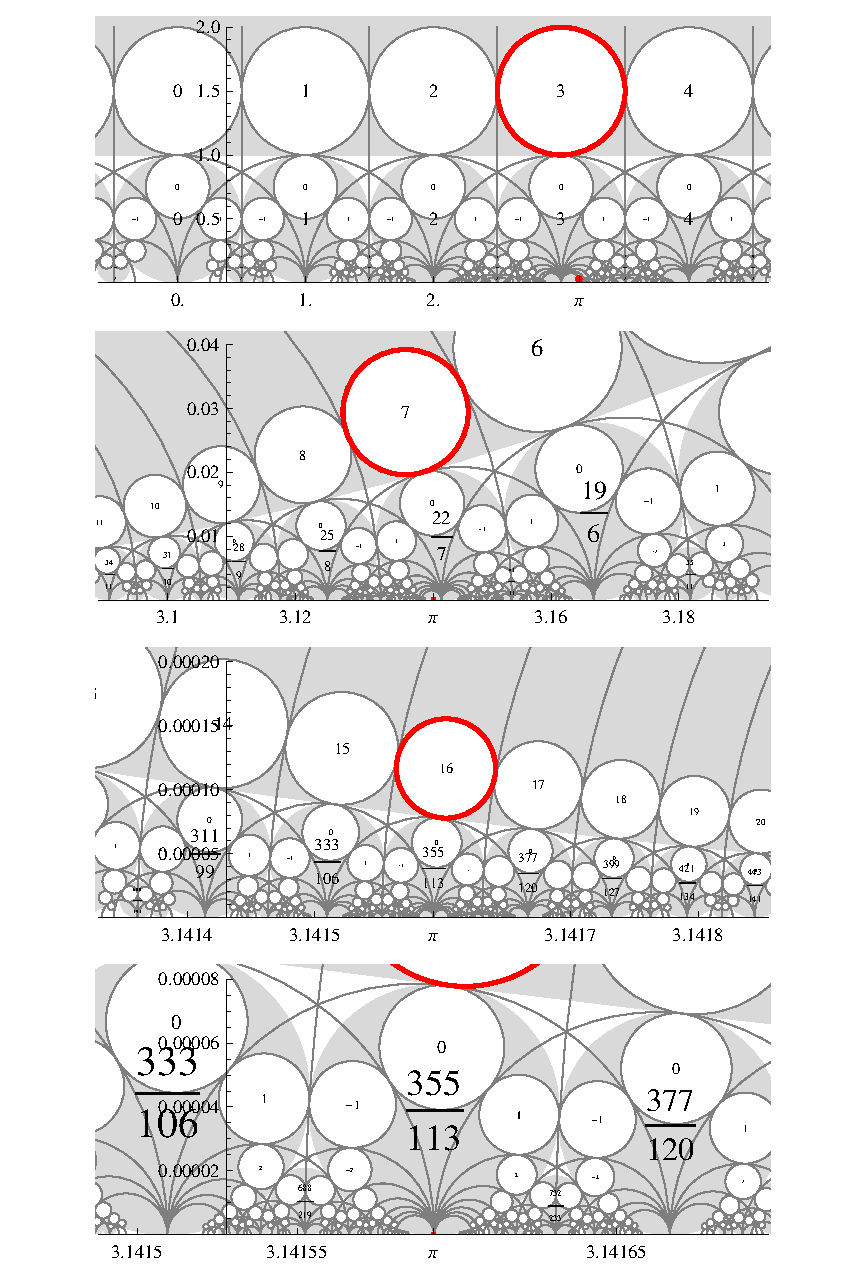
\includegraphics[width=\textwidth]{figures/cont-frac-pi}
\caption{$\pi = \frac{355}{113}$ -- well, almost.}
\label{fig_ContFracPi}
\end{figure}


\todo{19}{The modular group and ford circles}
